\documentclass[18pt, 4paper]{article}
\usepackage[ngerman]{babel}
\usepackage[T1]{fontenc}

\usepackage[utf8]{inputenc}
\usepackage{setspace}
\usepackage{amsmath}
\usepackage{amsfonts}
\usepackage{verbatim}
\usepackage{fancyhdr}
\usepackage{graphicx}
\usepackage[left=2cm, top=2cm, right=2cm, bottom=1.5cm]{geometry}
\usepackage{graphicx}
\usepackage{sidecap}
%\usepackage{polynom}
%\usepackage[yyyymmdd]{datetime}
%\renewcommand{\dateseparator}{}
%\usepackage{datetime2}

%\polyset{style=C}
\pagestyle{fancy} %eigener Seitenstil
\fancyhf{} %alle Kopf- und Fußzeilenfelder bereinigen
\fancyhead[L]{Differenzialrechnung-Funktionen} %Kopfzeile links
\fancyhead[C]{Fabian Pfaff} %zentrierte Kopfzeile
\fancyhead[R]{\today} %Kopfzeile rechts
\fancyfoot[L]{Differenzialrechnung-Funktionen} %Fußzeile links
\fancyhead[C]{Fabian Pfaff} %zentrierte Kopfzeile
\fancyfoot[C]{\thepage} %Seitennummer
\fancyfoot[R]{\today}
\renewcommand{\footrulewidth}{0.4pt} %untere Trennlinie

\begin{document}
\section*{Aufgabe1}
Es sei
\begin{math}
	f(x)=
	\left\{
	\begin{array}{cl}
		x	& \text{für $x<2$}\\
		x-2	& \text{für $x\geq2$ }
      	\end{array}
	\right.
\end{math}. Untersuchen sie $f(x)$ auf Stetigkeit.\\
\begin{figure}[h!]
	\centering
	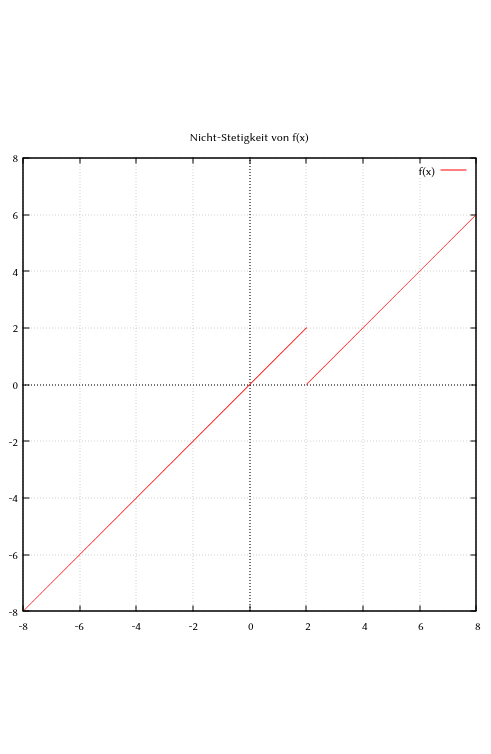
\includegraphics[scale=0.4]{images/unstetigkeit.png}
	\caption{Graph der Funktion f(x)}
\end{figure}
\hfill\\
Lineare Funktionen sind stetig. Deswegen muss die Stetigkeit für $x_0=2$\\
Eines der folgenden Argumente ist ausreichend.
 \begin{itemize}
	\item Der linksseitige Grenzwert $\lim_{x \to 2^+}{f(x)}$ beträgt 2, wohingegen der rechtseitige Grenzwert $\lim{x \to 2^-}{f(x)}$ beträgt 0.Da beide Werte in diesem Punkt nicht übereinstimmen ist die Funktion in $x_0=2$ nicht stetig
	\item Nach der $\epsilon-\delta$ Definition ist kein $\delta$ zu finden für $\epsilon < 0$. Somit ist die Funktion in $x_0=2$ nicht stetig.
\end{itemize}
\end{document}
